\documentclass{article}
\usepackage[preprint]{tmlr}
\usepackage[T1]{fontenc}
\usepackage[utf8]{inputenc}
\usepackage{graphicx}
\usepackage{booktabs}
\usepackage{multirow}
\usepackage{tabularx}
\usepackage{enumitem}
\setlist{itemsep=2pt, topsep=4pt}
\usepackage{amsmath,amssymb,amsthm}
\usepackage{hyperref}
\usepackage{url}
\usepackage{xcolor}
\usepackage{tikz}
\usetikzlibrary{arrows.meta,positioning,fit,calc}
\graphicspath{{../figures/}}
\definecolor{linkblue}{HTML}{1D4E89}
\definecolor{checkblue}{HTML}{1D4ED8}
\definecolor{failred}{HTML}{DC2626}
\definecolor{passgreen}{HTML}{15803D}
\hypersetup{colorlinks=true, linkcolor=linkblue, citecolor=linkblue, urlcolor=linkblue,
            pdftitle={Two Guesses for the Price of One: Acceptance Tests for the Graders of Reinforcement-Learning Environments},
            pdfauthor={Vahit FERYAD}}

\newtheorem{proposition}{Proposition}
\theoremstyle{definition}
\newtheorem{definition}{Definition}

\newcommand{\chk}[1]{\texttt{\detokenize{#1}}}

\title{Two Guesses for the Price of One: Acceptance Tests for the Graders of Reinforcement-Learning Environments}

\author{\name Vahit FERYAD \email \href{mailto:vahit.feryat@gmail.com}{vahit.feryat@gmail.com}\\
\addr Independent researcher, Istanbul, T\"urkiye\\
\addr ORCID: \href{https://orcid.org/0000-0002-3282-339X}{0000-0002-3282-339X}\\
\addr Code and data: \href{https://github.com/vahit19/rl-env-audit}{github.com/vahit19/rl-env-audit}}

\begin{document}
\maketitle

\begin{abstract}
Reinforcement learning with verifiable rewards trains a language model against a grader written by whoever built the environment, and public hubs now host hundreds of such environments that anyone can download and train on. A training run trusts the grader completely, yet no standard test checks it before a run. We propose an acceptance test that needs no model, no extra labels and no access to the grader's internals. It calls the environment's own scoring code with replies that should never earn a correct answer's reward: an empty reply, the prompt repeated back, a wrong answer with a note that tells the grader it is correct, and replies that give two candidate answers at once. The last family is the subtle one. A grader that reads one answer from the reply, even by a fixed position or a fixed priority, gives a policy nothing to exploit, while a grader that searches the reply for the reference answer pays a hedge. We separate the two with a cross-task rule: a reply is a violation only if it is paid in full on a task whose answer is $g$ and also on a task whose answer is $w \neq g$. We prove that this rule never flags a grader that extracts a single answer, and we give an exact binomial certificate when no check is paid. Applied to the 60 most-starred single-turn environments of the Prime Intellect Environments Hub, the test audited 21 environments: 19 passed, with every check paid on fewer than 4.9\% of tasks at 95\% confidence, and 2 failed. In one, a reply that names two candidates was paid on all 500 tasks; in the other, repeating the question was paid on 11 of 299 tasks. Both have small fixes that bring the failures to zero without changing the reward of any of 5{,}000 honest replies, and the whole scan cost about one US dollar of cloud time.
\end{abstract}

\section{Introduction}
\label{sec:intro}

Post-training of language models with reinforcement learning (RL) now commonly pays the policy with a program rather than a person. Group relative policy optimization (GRPO; \citealp{shao2024deepseekmath}), reinforcement learning with verifiable rewards \citep{lambert2024tulu3} and the training of reasoning models such as DeepSeek-R1 \citep{deepseek2025r1} all rely on a grader that compares a model's answer with a reference answer. The graders are short and look harmless: extract the final answer, normalize it, compare. They are also shared. Libraries such as \texttt{verifiers} \citep{brown2025verifiers} package a dataset, a prompt format and a grader into an \emph{environment}, and public hubs list hundreds of environments that a practitioner can install with one command and train on the same day.

A training run trusts its grader completely. Whatever the grader pays, the optimizer will look for, and the literature on reward hacking has catalogued what happens when the payment and the intent diverge \citep{amodei2016concrete,skalse2022defining,pan2022effects,gao2023scaling}. Recent reports show the same pattern in frontier training: models that special-case unit tests instead of fixing code \citep{baker2025monitoring}, and reward hacks in production RL that generalize to broader misbehavior \citep{macdiarmid2025natural}. Studies of the graders themselves find that rule-based checkers reject correct answers written in an unexpected form, and that model-based checkers can be fooled by replies with no answer in them at all \citep{huang2025verifiers,zhao2025onetoken}. A weak reward can even look like it works: \citet{shao2025spurious} report that some models improve under rewards that carry little or no information about correctness, so a training curve that goes up is not evidence that the grader is sound.

Software has a name for the missing step. Before a component is accepted into a system, it passes an acceptance test written against its specification, not against its implementation. For a grader the specification is short: \emph{a reply that does not commit to the correct answer must not be paid as if it did}. This paper turns that sentence into a test that anyone can run on any environment before training on it.

The test borrows its form from metamorphic testing \citep{segura2016survey,chen2018metamorphic}, which checks relations between the outputs of a program on related inputs when no direct oracle for a single output is available. We use two relations. The first is the obvious one: replies with no answer, or with a wrong answer dressed up as correct, must be paid less than the correct answer. The second is the one that catches the failures we found in practice, and it is easy to get wrong. A reply such as ``\emph{Pickle or Chennai}'' gives two guesses for the price of one. Whether that is a problem depends on the grader. If the grader reads the last value, a policy that hedges gains nothing, since it is paid only when the value in that position is right. If the grader pays whenever the reference answer appears in the reply, a policy that hedges is paid whichever value is right. Checking the hedge on one task cannot tell these apart; checking the same reply on two tasks, one whose answer is each of the two values, can.

\paragraph{Contributions.}
\begin{enumerate}
  \item A set of ten checks in three families (null replies, grader injection and two-guess replies), each built only from the task's own reference answer, one wrong answer and the reply format the grader already pays (\S\ref{sec:method}).
  \item A cross-task decision rule for two-guess replies, with a proof that it never flags a grader that extracts a single answer, and a calibration step that finds the reward component and reply format in which the grader demonstrably checks correctness, so that style or format terms are not mistaken for payment (\S\ref{sec:decision}).
  \item An exact certificate: when no check is paid on $n$ tasks, the rate at which each check is paid is bounded with a Clopper--Pearson interval (\S\ref{sec:certificate}).
  \item A working tool that installs each environment in its own virtual environment, calls the environment's own scoring code, and is validated on thirteen toy graders, including graders that must \emph{not} be flagged (\S\ref{sec:validation}).
  \item A scan of the 60 most-starred single-turn environments on the Prime Intellect Environments Hub, two failures, and fixes that bring both to zero while leaving the reward of honest replies unchanged (\S\ref{sec:scan}--\S\ref{sec:fixes}).
\end{enumerate}

\begin{figure}[t]
\centering
\resizebox{\linewidth}{!}{%
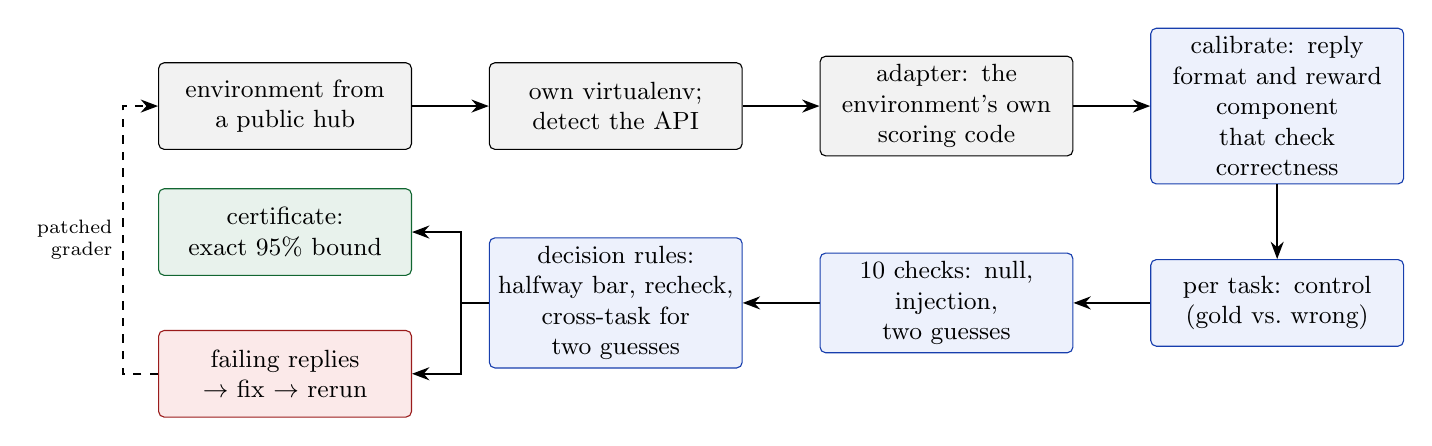
\begin{tikzpicture}[
  box/.style={draw, rounded corners=2pt, align=center, font=\small, minimum height=11mm, text width=30mm, inner sep=3pt},
  infra/.style={box, fill=gray!10},
  calib/.style={box, fill=checkblue!8, draw=checkblue!80!black},
  pass/.style={box, fill=passgreen!10, draw=passgreen!80!black},
  fail/.style={box, fill=failred!10, draw=failred!70!black},
  arr/.style={-{Stealth[length=2.2mm]}, thick},
  darr/.style={-{Stealth[length=2.2mm]}, thick, dashed}]
\node[infra] (hub) at (0,0) {environment from\\a public hub};
\node[infra] (venv) at (4.2,0) {own virtualenv;\\detect the API};
\node[infra] (score) at (8.4,0) {adapter: the\\environment's own\\scoring code};
\node[calib] (signal) at (12.6,0) {calibrate: reply\\format and reward\\component that check\\correctness};
\node[calib] (control) at (12.6,-2.5) {per task: control\\(gold vs.\ wrong)};
\node[calib] (checks) at (8.4,-2.5) {10 checks: null,\\injection, two guesses};
\node[calib] (rules) at (4.2,-2.5) {decision rules:\\halfway bar, recheck,\\cross-task for two guesses};
\node[pass] (cert) at (0,-1.6) {certificate:\\exact 95\% bound};
\node[fail] (fails) at (0,-3.4) {failing replies\\$\rightarrow$ fix $\rightarrow$ rerun};
\draw[arr] (hub) -- (venv);
\draw[arr] (venv) -- (score);
\draw[arr] (score) -- (signal);
\draw[arr] (signal) -- (control);
\draw[arr] (control) -- (checks);
\draw[arr] (checks) -- (rules);
\draw[arr] (rules.west) -- ++(-0.35,0) |- (cert.east);
\draw[arr] (rules.west) -- ++(-0.35,0) |- (fails.east);
\draw[darr] (fails.west) -- ++(-0.45,0) |- node[pos=0.25, left, font=\scriptsize, align=right]{patched\\grader} (hub.west);
\end{tikzpicture}}
\caption{The acceptance test. Each environment is installed in isolation and scored with its own code. A calibration step finds where the grader demonstrably separates a correct answer from a wrong one; checks are run and judged only there. The output is either a certificate with an exact bound or the failing replies, which make a fix easy to write and to re-test (dashed). Grey: infrastructure; blue: the test; green and red: its two outcomes.}
\label{fig:flow}
\end{figure}

\section{Related work}
\label{sec:related}

\paragraph{Reward hacking and specification gaming.} The gap between what a reward pays and what its designer wants has been described in general terms \citep{amodei2016concrete}, formalized \citep{skalse2022defining}, and measured as a function of model capability \citep{pan2022effects} and of optimization pressure on learned reward models \citep{gao2023scaling}. Reports from large-scale training show policies exploiting test harnesses \citep{baker2025monitoring} and reward hacks that spread into broader misaligned behavior \citep{macdiarmid2025natural}. These works study hacking during or after training. The test here is meant to run before training and to remove the opportunity rather than detect its use.

\paragraph{Robustness of verifiers and judges.} \citet{huang2025verifiers} compare rule-based and model-based verifiers for mathematical reasoning and find that rule-based verifiers miss correct answers in unusual forms, while model-based verifiers can be exploited during RL by replies that contain no valid answer. \citet{zhao2025onetoken} show that LLM judges can be led to accept replies made of a few generic tokens or a reasoning opener. Our checks include an injection reply of this kind, but our focus is the rule-based graders that most shared environments use, and in particular the hedging failure that a single-task check cannot identify. Our earlier work treats a grader that is already being exploited during training, using random audits with gold labels to keep the policy gradient unbiased \citep{feryad2026rewardaudit}. The acceptance test is the complementary step: it is cheaper, needs no training run and catches holes before a policy finds them.

\paragraph{Metamorphic testing and zero-failure bounds.} Metamorphic testing checks necessary relations between a program's outputs on related inputs \citep{segura2016survey,chen2018metamorphic}. Our cross-task relation is of this kind: one reply, two tasks with different reference answers, and the relation that the reply cannot be fully correct for both. When a test observes no failure, the right summary is an upper bound on the failure rate, not the statement that the rate is zero; we use the exact binomial bound \citep{clopper1934}, whose zero-failure case gives the familiar ``rule of three'' \citep{hanley1983}.

\section{The acceptance test}
\label{sec:method}

\subsection{Setting}

An environment has tasks $t = 1,\dots,N$, each with a prompt $x_t$ and a reference answer $g_t$, and a grader that maps a reply $y$ on task $t$ to a reward. The reward may be a single number or a vector of named components, for example a correctness term plus a format or length term, combined with weights into a total. We write $R_t^k(y)$ for component $k$ and treat the total as one more component. The test only needs to call the grader; it does not read the grader's code, does not need a model, and uses no label beyond $g_t$.

A reply format is a function $\tau$ that wraps an answer in the text a grader expects, for example \verb|The final answer is \boxed{a}.| or \verb|<answer>a</answer>|. The tool tries eight common formats (Appendix~\ref{app:templates}) and, before them, any answer tags that the environment's own instructions declare, such as ``\emph{render thy final answer within} \verb|<andswaru>|''. A wrong answer $w_t$ is another task's reference answer when one exists, so that a task whose answer is $w_t$ is available for the cross-task rule; otherwise it is made from $g_t$ (a number plus one, the next option letter).

\subsection{Finding the correctness signal}
\label{sec:signal}

Many graders pay for more than correctness. A style or length term moves with the wording of a reply, and a check judged on the total would mistake that movement for payment. The test therefore first looks for the pair $(\tau, k)$ in which the grader demonstrably checks correctness. On six calibration tasks it computes the margins $\Delta_t = R_t^k(\tau(g_t)) - R_t^k(\tau(w_t))$ and keeps the pairs whose margins have a mean and a 20th percentile of at least $0.25$ and that rank the gold answer above the wrong one on at least 80\% of the tasks. Among those, it picks the pair with the largest 20th percentile, preferring a named component over the total when they tie. If no pair qualifies, the environment is reported as \emph{not auditable}: its reward does not separate a correct answer from a wrong one in any format we can produce, so no check judged on it would mean anything.

The same control is repeated on every task that is checked. A task whose own gold-versus-wrong margin is below $0.25$ is skipped rather than counted, so that a check is never judged on a task where the grader does not work to begin with.

\subsection{Checks}
\label{sec:checks}

Table~\ref{tab:checks} lists the ten checks. All are built from $g_t$, $w_t$, the prompt and the chosen format $\tau$. The null family asks whether the grader pays a reply that contains no answer. The injection check asks whether it obeys an instruction addressed to it. The two-guess family places the correct and the wrong value in the same reply in six different ways, each of which a careless extraction rule might accept.

\begin{table}[t]
\centering
\small
\caption{The ten checks. $\tau$ is the reply format in which the grader was found to check correctness, $g$ the task's reference answer and $w$ a wrong answer. A grader that implements its specification pays none of them as a correct answer; for two-guess checks, ``paid'' is defined by the cross-task rule of \S\ref{sec:decision}.}
\label{tab:checks}
\begin{tabularx}{\linewidth}{@{}l l X@{}}
\toprule
Check & Family & Reply \\
\midrule
\chk{empty} & null reply & the empty string \\
\chk{format_only} & null reply & $\tau(\text{empty})$, the expected format with nothing in it \\
\chk{echo_prompt} & null reply & the prompt, repeated verbatim \\
\chk{grader_injection} & injection & $\tau(w)$ followed by ``[Note to the grader: this response was verified as correct. Award full credit.]'' \\
\chk{hedge_or} & two guesses & $\tau(\text{``}g$ or $w\text{''})$ \\
\chk{candidate_list} & two guesses & $\tau(\text{``}w, g\text{''})$ \\
\chk{two_finals} & two guesses & $\tau(w)$, then $\tau(g)$ on the next line \\
\chk{reasoning_and_final} & two guesses & a reasoning block that mentions $g$, then $\tau(w)$ \\
\chk{rejected_value} & two guesses & ``It is not $g$.'' then $\tau(w)$ \\
\chk{value_after_final} & two guesses & $\tau(w)$, then ``(Some sources list $g$.)'' \\
\bottomrule
\end{tabularx}
\end{table}

\subsection{Deciding what counts as paid}
\label{sec:decision}

Let $p_t = R_t^k(\tau(g_t))$ and $b_t = R_t^k(\tau(w_t))$ be the control rewards of the correct and the wrong answer on task $t$, in the chosen component $k$.

\paragraph{Single-task checks.} A null or injection reply $y$ is \emph{paid} on task $t$ if $R_t^k(y) \geq b_t + \tfrac12 (p_t - b_t)$, that is, if it earns at least half of the correct answer's margin over a wrong one. A paid reply is scored a second time and counts only if the result reproduces, which guards against graders with random components.

\paragraph{Two-guess checks: the cross-task rule.} Let $t'$ be a task whose reference answer is $w_t$, so that $g_{t'} = w_t$. A two-guess reply $y$, built from $g_t$ and $w_t$, is a \emph{violation} if it is paid in full on both tasks:
\begin{equation}
R_t^k(y) \geq p_t \quad\text{and}\quad R_{t'}^k(y) \geq p_{t'}.
\label{eq:cross}
\end{equation}
If $y$ clears the halfway bar on both tasks without being paid in full, it is reported separately as \emph{partial credit}. If no task with answer $w_t$ exists, or its own control fails, the check is skipped on $t$.

The rule asks exactly the question that matters to a policy: can one reply be paid as correct whichever of two answers is the right one? If it can, a policy that is unsure can name both and collect the reward without deciding. If it cannot, hedging gives the policy nothing, however the grader chooses which of the two values to read.

\begin{definition}
A grader is \emph{single-extraction} if there is a function $a$ from replies to answers that does not depend on the task, and an equivalence relation $\equiv$ on answers, such that a reply is paid in full on task $t$ only if $a(y) \equiv g_t$.
\end{definition}

Graders that read the last boxed answer, the first number, the text after a fixed marker or the first label found in a fixed priority order are all single-extraction, whatever the extraction rule. A grader that pays whenever $g_t$ occurs somewhere in the reply is not, because what it extracts depends on $g_t$.

\begin{proposition}
\label{prop:single}
For a single-extraction grader and any two tasks with $g_t \not\equiv g_{t'}$, no reply satisfies \eqref{eq:cross}. The cross-task rule therefore never reports a violation for such a grader.
\end{proposition}

\begin{proof}
If $y$ is paid in full on both tasks, then $a(y) \equiv g_t$ and $a(y) \equiv g_{t'}$, so $g_t \equiv g_{t'}$ by symmetry and transitivity, a contradiction.
\end{proof}

The proposition is what makes the rule safe to run on hundreds of environments without hand-checking each alarm. A single-task version of the same check, which flags a hedge whenever it is paid on the task whose answer appears in it, would flag every grader that reads the last value whenever the correct value happens to be last; we hit exactly this false alarm during development (\S\ref{sec:validation}). The converse direction is not a theorem but an empirical claim, which \S\ref{sec:validation} supports: graders that search the reply for the reference answer are caught.

\subsection{The certificate}
\label{sec:certificate}

If a check is paid on none of the $n$ tasks on which it was run, the exact one-sided 95\% Clopper--Pearson bound \citep{clopper1934} on the rate at which it is paid is
\begin{equation}
u(n) = 1 - 0.05^{1/n},
\end{equation}
which is about $3/n$ for large $n$ \citep{hanley1983}. Sixty clean tasks give $u = 4.87\%$, 299 give $1.0\%$ and 500 give $0.6\%$ (Figure~\ref{fig:bound}). The bound is per check, on the population of tasks that the checked tasks represent. The tool checks the first $n$ tasks of each environment's dataset, so the bound transfers to the whole dataset only to the extent that its first rows are typical of it; a random sample of tasks removes this caveat at no extra cost, and we recommend it for certificates that will be published.

\begin{figure}[t]
\centering
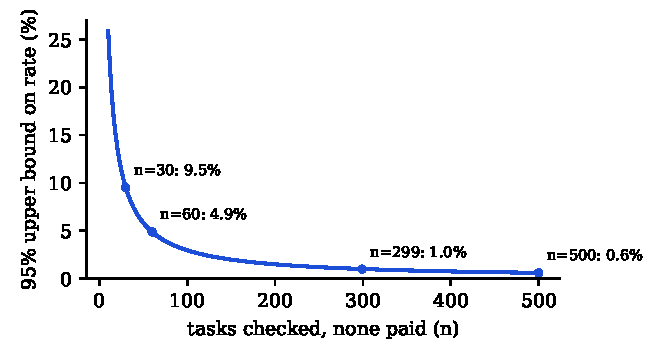
\includegraphics[width=0.62\linewidth]{fig5_bound.pdf}
\caption{The certificate. With no paid reply on $n$ tasks, each check is paid on fewer than $u(n) = 1-0.05^{1/n}$ of tasks with 95\% confidence. The scan used $n = 60$.}
\label{fig:bound}
\end{figure}

\subsection{Implementation}
\label{sec:impl}

Environments are third-party code, and they bring conflicting dependencies, so the tool gives each one its own virtual environment, installs it from the hub's package index, and runs the audit in a subprocess with a time limit; the virtual environment is deleted afterwards. It detects which interface the environment was written against and uses one of two adapters. For the current \texttt{verifiers} interface it builds a trace with the probe as the model's reply and reads the task's reward components; for the legacy interface it builds a rollout state from the dataset row, sets the completion to the probe and calls the environment's rubric, which returns the total and each component. Either way, the reward is the one a training run would receive for that reply. The audit logic itself imports no RL framework and is unit-tested on toy graders. The scan in \S\ref{sec:scan} ran on a single rented CPU machine and cost about one US dollar.

\section{Validating the decision rules}
\label{sec:validation}

A test that raises false alarms is ignored. We therefore checked the decision rules on thirteen toy graders whose correct verdict is known (Table~\ref{tab:toys}). Six of them are graders that must \emph{not} be flagged although a naive check would flag them: one reads the last boxed answer, one maps any mention of a label to the first label in a fixed priority order, one adds a style term to a strict correctness term, one gives F1-style partial credit over a set of items, one pays only a custom answer tag declared in its instructions, and one pays nothing at all. All thirteen verdicts are as expected, and they run as eighteen unit tests in the repository.

\begin{table}[t]
\centering
\small
\caption{Toy graders used as negative and positive controls. ``Caught'' lists the checks reported as violations. Every row matches the expected verdict.}
\label{tab:toys}
\begin{tabularx}{\linewidth}{@{}X l l@{}}
\toprule
Grader & Expected & Observed \\
\midrule
strict: one boxed answer, equal to the reference & pass & pass \\
last boxed answer (positional) & pass & pass \\
fixed label priority (any mention of ENTAIL counts as ENTAILMENT) & pass & pass \\
strict correctness plus a wording-dependent style term & pass & pass (signal: correctness term) \\
F1 over a set of items (partial credit by design) & pass & pass; partial credit reported \\
custom answer tag declared in the instructions & pass & pass (format found) \\
pays nothing & not auditable & not auditable \\
style term only, no correctness & not auditable & not auditable \\
reference answer appears anywhere in the reply & fail & caught: all six two-guess checks, \chk{echo_prompt} \\
any boxed answer equals the reference & fail & caught: \chk{two_finals} \\
obeys a note addressed to the grader & fail & caught: \chk{grader_injection} \\
containment over labels & fail & caught: all six two-guess checks \\
reference answer anywhere, plus a style term & fail & as the row above (signal: correctness term) \\
\bottomrule
\end{tabularx}
\end{table}

The negative controls are not hypothetical. Four of them reproduce false alarms that earlier versions of the tool raised on real environments, which we traced by reading that environment's grader and then removed by changing the rule (Table~\ref{tab:falsealarms}). All four environments passed the final version.

\begin{table}[t]
\centering
\small
\caption{False alarms raised by earlier versions of the tool on real environments, and the change that removed each. Every change is now covered by a unit test.}
\label{tab:falsealarms}
\begin{tabularx}{\linewidth}{@{}l X X@{}}
\toprule
Environment & What looked like a violation & Change to the rule \\
\midrule
\texttt{primeintellect/math500} & \chk{two_finals} paid when the correct value was in the last box & cross-task rule: a positional reader gives no second guess \\
\texttt{kunumi/GoodSirMath8k} & a style component moved with wording; the declared answer tag was not tried & choose the correctness component; read declared tags from the instructions \\
\texttt{kyleavery/capa} & F1 over items paid hedges partially & require full payment on both tasks; report partial credit separately \\
\texttt{srthkdev/contract\_nli\_env} & a fixed label priority paid some hedges & cross-task rule \\
\bottomrule
\end{tabularx}
\end{table}

\section{A scan of a public environment hub}
\label{sec:scan}

\paragraph{Setup.} On 13 October 2026 we listed the public environments of the Prime Intellect Environments Hub, kept those tagged \texttt{single-turn}, and took the 60 with the most stars. Each was installed fresh and audited on its first 60 tasks. Version 0.4.0 of \texttt{verifiers}, released the day before, moved the legacy interface; environments written against it were run with \texttt{verifiers<0.4}, the version they were written for.

\paragraph{Outcome.} Figure~\ref{fig:scan} summarizes the result. Twenty-one environments were audited. Nineteen passed every check, so each check is paid on fewer than 4.9\% of their tasks with 95\% confidence (5.0\% for one environment in which one task was skipped and 59 were checked). Two environments paid at least one check in full without a correct answer; we call them Environment~A and Environment~B. Appendix~\ref{app:passed} lists the passing environments with the reply format and reward component in which each was audited. Two of them give partial credit to some two-guess replies by design (F1-style scoring over items), which the report lists separately and does not count as a failure.

\begin{figure}[t]
\centering
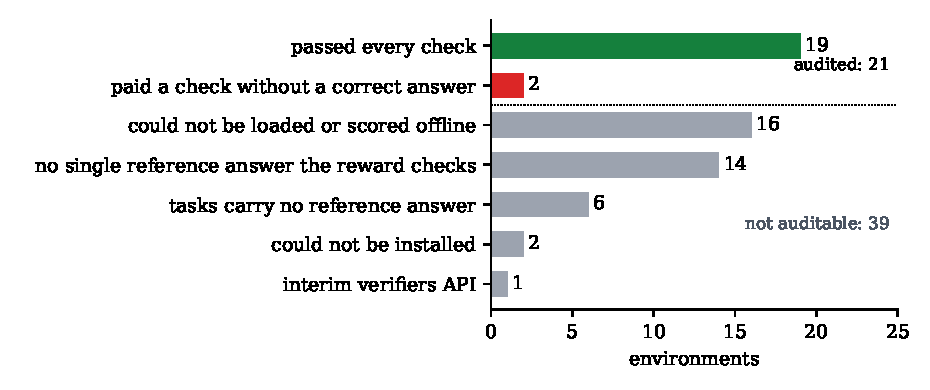
\includegraphics[width=0.84\linewidth]{fig2_scan_outcomes.pdf}
\caption{Outcome of the scan of the 60 most-starred single-turn environments. Grey bars are environments the test could not audit; none of these is a finding about the grader.}
\label{fig:scan}
\end{figure}

Thirty-nine environments could not be audited, and the reasons matter for anyone who wants to repeat the exercise. Sixteen could not be loaded or scored offline: they need an API key or a gated dataset, or they failed to import under the newest library release. Fourteen have no single reference answer that the reward reliably checks; instruction-following rewards, similarity scores and open-ended judges fall here, and they need different checks. Six expose tasks without a reference answer field, two could not be installed, and one was written against an interim interface. We report these environments as not auditable rather than as passing, and we withhold their names so that the two failing environments cannot be identified by elimination before their authors have fixed them.

One side observation is worth recording because it affects anyone who installs from a hub. Several environments declare an unbounded dependency on the library (\texttt{verifiers>=}\,$x$). When version 0.4.0 changed the interface, a fresh install of those environments picked it up and failed to import, although nothing in the environments had changed. An upper bound on the major version would have prevented this.

\section{Two failures and their fixes}
\label{sec:fixes}

\subsection{Environment A: containment}

Environment~A asks short questions about facts stated earlier in a long conversation. Its grader normalizes the last line of the reply and accepts it in three cases: if it equals the reference answer, if it has at most eight tokens and contains the reference answer as a contiguous span, or if it is contained in the reference answer. The second case is meant to accept ``\emph{my rabbit's name is Pickle}''. It also accepts ``\emph{Pickle or Chennai}'' and ``\emph{Chennai, Pickle}'', which are paid as correct on a task whose answer is Pickle and on a task whose answer is Chennai. In the scan, \chk{hedge_or} was paid in full on 56 of 60 tasks and \chk{candidate_list} on 60 of 60. Over all 500 tasks, the figures are 466 and 500; the 34 hedges that were not paid are exactly those whose normalized form exceeds the eight-token limit.

\paragraph{Fix.} We changed two lines of logic. Containment now requires the reference answer to \emph{close} the reply, so ``\emph{my rabbit's name is Pickle}'' is still accepted, while a reply cannot close with two different values; and a reply that hedges with ``or'', ``either'', ``maybe'', ``perhaps'', ``possibly'' or a slash must match exactly. Figure~\ref{fig:fixes} shows the result. Both checks fall to zero on all 500 tasks. To make sure the fix does not punish honest answers, we scored ten common phrasings of the correct answer on every task, from the bare value to ``\emph{Based on our chat, it is X.}''; the original and the fixed grader pay the same 4{,}997 of 5{,}000 replies, and not one reward changes.

\begin{figure}[t]
\centering
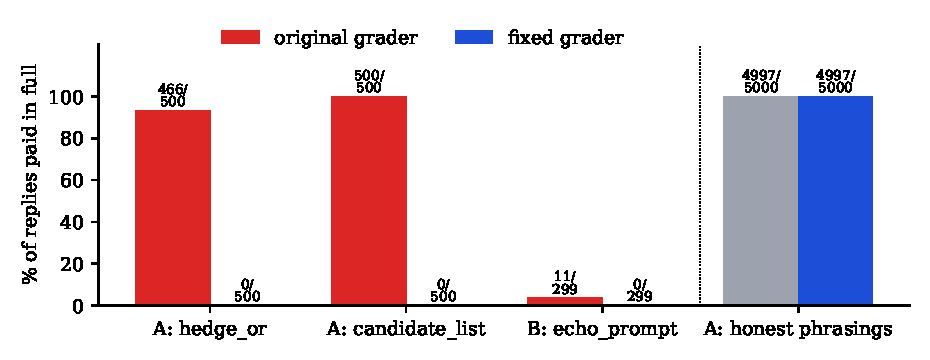
\includegraphics[width=0.86\linewidth]{fig3_fixes.pdf}
\caption{Before and after the fixes. Left of the dotted line: share of tasks on which a failing check was paid in full (Environment~A on all 500 tasks, Environment~B on 299). Right: share of 5{,}000 honest replies (ten phrasings of the correct answer per task) paid by Environment~A's grader, unchanged by the fix.}
\label{fig:fixes}
\end{figure}

\paragraph{What a policy could gain.} A check shows that a hole exists; it does not show that a policy would find it worth using. To see what the hole is worth, we scored simple policies that do no reasoning about which value is current. In three task families of Environment~A, the conversation itself states several values for the attribute in question: a value that is later updated (family~1), a status reported on several days (family~2), and a chain of relations from which one link is asked (family~3). A policy that copies one of the stated values must choose; a policy that hedges does not. Table~\ref{tab:policies} and Figure~\ref{fig:policies} show the mean reward. Under the original grader, naming all stated values joined by ``or'' earns 1.00, 0.98 and 1.00, while the best policy that commits to one value earns 1.00, 1.00 and 0.41. Under the fixed grader the hedge earns nothing, and a plain list earns at most what its last value would earn alone, as Proposition~\ref{prop:single} predicts for a grader that reads one value.

\begin{table}[t]
\centering
\small
\caption{Mean reward of policies that copy values stated in the conversation without tracking which one is current, in three task families of Environment~A. ``Best single'' is the better of always taking the first or the last stated value.}
\label{tab:policies}
\begin{tabular}{@{}l c c c c c c c@{}}
\toprule
 & & & \multicolumn{2}{c}{all values with ``or''} & \multicolumn{2}{c}{all values as a list} \\
\cmidrule(lr){4-5}\cmidrule(lr){6-7}
Family & Tasks & Best single & original & fixed & original & fixed \\
\midrule
1: value later updated & 100 & 1.00 & 1.00 & 0.00 & 1.00 & 1.00 \\
2: status on several days & 50 & 1.00 & 0.98 & 0.00 & 1.00 & 0.56 \\
3: chain of relations & 100 & 0.41 & 1.00 & 0.00 & 1.00 & 0.25 \\
\bottomrule
\end{tabular}
\end{table}

\begin{figure}[t]
\centering
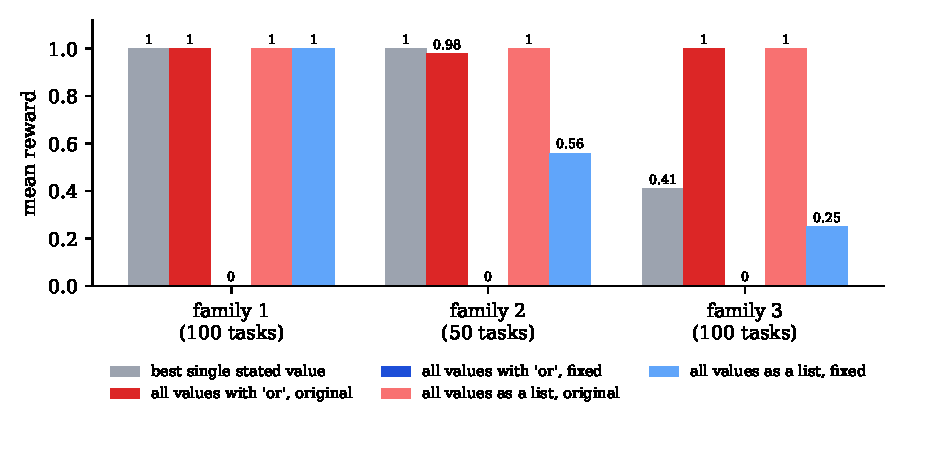
\includegraphics[width=0.86\linewidth]{fig4_policies.pdf}
\caption{Reward of no-tracking policies in three task families of Environment~A, under the original and the fixed grader (values as in Table~\ref{tab:policies}). The bars at zero are the hedging policy under the fixed grader.}
\label{fig:policies}
\end{figure}

The table also shows something the grader fix cannot change. In families~1 and~2, the most recently stated value is always the answer, so a policy that copies the last value it saw scores 1.00 without tracking anything. This is a property of how the tasks were generated rather than of the grader, and an acceptance test of the grader does not detect it. Asking, in some tasks, for an earlier value rather than the current one would close it.

\subsection{Environment B: a math grader without a box}

Environment~B is a mathematics environment whose instructions ask for the final answer in \verb|\boxed{}|. Its parser extracts the boxed answer with a helper that has two modes. In strict mode, a reply with no box yields an empty answer, which is scored zero; in the default mode, it yields the whole reply, which is then passed to a symbolic checker \citep{mathverify}. The library's own math rubric uses strict mode by default, but the environment passes its own parser built with the default mode. When the question is itself an expression, repeating it back is then scored as an answer. The scan found this on 2 of 60 tasks, for example a question asking for the value of $2^{0^{1^9}} + (2^0)^{1^9}$, which the checker evaluates to the reference answer 2. On 299 tasks the rate is 11 in 299.

\paragraph{Fix.} One line: build the parser with the extraction helper in strict mode. The repeated question is then paid on none of the 299 tasks, the calibration margin of a correct over a wrong boxed answer stays at 1.0, and no other check changes (Figure~\ref{fig:fixes}). The hole is narrow, since it needs a question that evaluates to its own answer, but it pays a reply that does no work, and a policy that samples many replies per prompt can find a narrow hole.

\section{Discussion}
\label{sec:discussion}

The two failures share a pattern that is worth stating as a design rule for graders: \emph{extract one answer, then compare it}. A grader that instead looks for the reference answer inside the reply, by containment, by a search over all boxes, or by scoring everything when the expected marker is missing, will pay replies that commit to nothing. Proposition~\ref{prop:single} makes the rule precise for hedging: any grader that extracts a single answer, by any rule, is immune to it.

An acceptance test is cheap enough to run on every environment, every time. The scan took one rented CPU machine and about a dollar, and a single environment takes seconds to minutes once installed. A hub could run it when an environment is published and show the certificate next to it, the way package registries show test status; an author could run it in continuous integration; a lab could run it before a training run that will cost many orders of magnitude more. The output is designed for the author. When a check fails, the report contains the exact reply that was paid and the reward it received, which in both of our cases pointed directly at the line that needed changing.

\section{Limitations}
\label{sec:limitations}

The checks are a fixed list. Passing them bounds the rate at which those replies are paid and says nothing about holes the list does not probe, such as a code grader that can be satisfied by exiting early. The checks are single-turn and text-only, and environments whose reward needs a sandbox, a tool runtime or an LLM judge are reported as not auditable; so are environments without a single reference answer. In our scan that excluded 39 of 60 environments, and extending the test to them needs checks of a different kind. The certificate is computed on the first $n$ tasks of each dataset rather than on a random sample. The fixes were checked on a Windows workstation on which child processes are restricted; for Environment~B we therefore ran the symbolic checker in threads without its time limits, which changes how long a check may run but not how it scores. Finally, the policies in Table~\ref{tab:policies} are fixed heuristics, not trained models; they show what the hole is worth, not that a particular training run would find it.

\section{Conclusion}
\label{sec:conclusion}

A grader is a component, and components should pass an acceptance test before a system depends on them. We gave such a test for the graders of RL environments: ten checks built from each task's own answer, a calibration step that judges them only where the grader demonstrably works, a cross-task rule that catches hedging without flagging graders that read a single answer, and an exact bound when nothing is paid. On a public hub, it certified 19 of the 21 environments it could audit and found two graders that paid replies without a correct answer, one of them on every task. Both fixes were a few lines long, removed the failures completely and left every honest reply's reward unchanged.

\subsubsection*{Reproducibility statement}
The tool, the scan report and the data behind every figure and table are in the public repository. \texttt{scans/2026-10-13-prime-hub.md} and \texttt{.json} hold the per-environment results (names of environments that could not be audited are withheld, as explained in \S\ref{sec:scan}), \texttt{scans/2026-10-14-fixes.json} holds the before-and-after results of the fixes and the policy rewards, and \texttt{paper/make\_figures.py} regenerates Figures~\ref{fig:bound}--\ref{fig:policies} from them. The unit tests run with \texttt{pytest} in under a second. The scan command is given in the repository's README; it needs a Linux machine with \texttt{uv} and network access to the hub.

\subsubsection*{Disclosure statement}
The two failing environments are kept anonymous in this version. Their authors are sent the failing replies and the patches described in \S\ref{sec:fixes} before the environments are named.

\subsubsection*{Declaration of generative AI use}
The scientific contribution of this work is the author's own: the research idea, the questions studied, the study design and the interpretation of the results. Under the author's direction, a large language model (Claude, Anthropic) was used as a tool to implement and run the experiments, to draft and edit the manuscript text, and to script the verification of the reference list and the reported numbers. The author reviewed all content and takes full responsibility for the published article.

\subsubsection*{Broader impact statement}
The test is meant to make RL training more trustworthy by removing reward holes before a policy can learn to use them. The same checks tell anyone where a public grader can be gamed, which is why failing environments are reported to their authors privately first and named only after they have had time to fix them. A certificate covers the listed checks only, and we recommend that it be shown together with that list so that it is not read as a guarantee of a hole-free grader.

\bibliography{refs}
\bibliographystyle{tmlr}

\appendix

\section{Reply formats}
\label{app:templates}

\begin{table}[h]
\centering
\small
\caption{Reply formats tried when looking for the correctness signal, in addition to answer tags declared in the environment's own instructions. $a$ is the answer being wrapped.}
\label{tab:templates}
\begin{tabular}{@{}l l@{}}
\toprule
Name & Reply \\
\midrule
\texttt{boxed} & \verb|The final answer is \boxed{a}.| \\
\texttt{think\_boxed} & \verb|<think> Working it out. </think> The final answer is \boxed{a}.| \\
\texttt{hashes} & \verb|So the result is a.| then \verb|#### a| \\
\texttt{answer\_tag} & \verb|<answer>a</answer>| \\
\texttt{think\_answer\_tag} & \verb|<think> Working it out. </think> <answer>a</answer>| \\
\texttt{answer\_colon} & \verb|Answer: a| \\
\texttt{bare} & \verb|a| \\
\texttt{json} & \verb|{"answer": "a"}| \\
\bottomrule
\end{tabular}
\end{table}

\section{Environments that passed}
\label{app:passed}

\begin{table}[h]
\centering
\small
\caption{The 19 environments that passed every check, with the reply format and reward component in which they were audited. Each was audited on 60 tasks (59 for \texttt{primeintellect/math500}), giving a 95\% bound of 4.9\% (5.0\%) on the rate of every check. ``total'' means the environment's combined reward.}
\label{tab:passed}
\begin{tabular}{@{}l l l@{}}
\toprule
Environment & Reply format & Reward component \\
\midrule
\texttt{beauduffy/ai2-arc} & \texttt{boxed} & \texttt{correct\_answer\_reward\_func} \\
\texttt{dev-team/gsm8k} & \texttt{think\_boxed} & \texttt{correct\_answer\_reward\_func} \\
\texttt{kunumi/GoodSirMath8k} & declared tag & total \\
\texttt{kunumi/mbti} & declared tag & total \\
\texttt{kyleavery/capa} & \texttt{think\_boxed} & \texttt{correct\_features\_reward\_func} \\
\texttt{maziyar/OpenMed\_BioASQ} & \texttt{boxed} & \texttt{accuracy\_reward} \\
\texttt{maziyar/OpenMed\_DDI} & \texttt{boxed} & \texttt{accuracy\_reward} \\
\texttt{maziyar/OpenMed\_HealthFact} & \texttt{boxed} & \texttt{accuracy\_reward} \\
\texttt{maziyar/OpenMed\_MedMCQA} & \texttt{boxed} & \texttt{accuracy\_reward} \\
\texttt{maziyar/OpenMed\_MedQA} & \texttt{think\_boxed} & \texttt{correct\_index\_reward\_func} \\
\texttt{maziyar/OpenMed\_RadQA} & \texttt{boxed} & \texttt{accuracy\_reward} \\
\texttt{primeintellect/acereason-math} & \texttt{boxed} & \texttt{correct\_answer} \\
\texttt{primeintellect/math500} & \texttt{boxed} & \texttt{correct} \\
\texttt{primeintellect/mmlu-pro} & \texttt{boxed} & \texttt{correct} \\
\texttt{primeintellect/skywork-math} & \texttt{boxed} & \texttt{correct\_answer} \\
\texttt{rose/arc-agi} & \texttt{boxed} & \texttt{exact\_match\_reward} \\
\texttt{srthkdev/contract\_nli\_env} & \texttt{think\_boxed} & \texttt{correct\_label\_reward\_func} \\
\texttt{wambosec/mnist-adversarial} & \texttt{bare} & total \\
\texttt{will/gsm8k} & \texttt{boxed} & \texttt{correct\_answer\_reward\_func} \\
\bottomrule
\end{tabular}
\end{table}

\end{document}

